%
% File emnlp2018.tex
%
%% Based on the style files for EMNLP 2018, which were
%% Based on the style files for ACL 2018, which were
%% Based on the style files for ACL-2015, with some improvements
%%  taken from the NAACL-2016 style
%% Based on the style files for ACL-2014, which were, in turn,
%% based on ACL-2013, ACL-2012, ACL-2011, ACL-2010, ACL-IJCNLP-2009,
%% EACL-2009, IJCNLP-2008...
%% Based on the style files for EACL 2006 by 
%%e.agirre@ehu.es or Sergi.Balari@uab.es
%% and that of ACL 08 by Joakim Nivre and Noah Smith

\documentclass[11pt,a4paper]{article}
  \usepackage[hyperref]{emnlp2018}
  \usepackage{times}
  \usepackage{latexsym}
  
  \usepackage{url}
  
  \usepackage{graphicx}
  
  \aclfinalcopy % Uncomment this line for the final submission
  
  %\setlength\titlebox{5cm}
  % You can expand the titlebox if you need extra space
  % to show all the authors. Please do not make the titlebox
  % smaller than 5cm (the original size); we will check this
  % in the camera-ready version and ask you to change it back.
  
  \newcommand\BibTeX{B{\sc ib}\TeX}
  \newcommand\confname{EMNLP 2018}
  \newcommand\conforg{SIGDAT}
  
  \title{Visual Active Learning for Relation Extraction}
  
  \author{Kairong Jiang \\
    University of Arizona \\
    {\tt jiangkairong@email.arizona.edu}\\\And
    Mihai Surdeanu \\
    University of Arizona\\}
  
  \date{}
  
  \begin{document}
  \maketitle
  
  \section{Introduction}
  Relation extraction is an import part of information extraction (IE) where a classifier is trained to label the \emph{relation} between a set of entity mentions in some text. It provides crucial information for later IE processes like disambiguation. For example, in the sentence ``\textbf{Obama} \emph{was born in} the \textbf{United States} just as he has always said.'', the classifier should label relation \emph{``BornIn''} with entity mention pair ``Barack Obama'' and ``United States''.

  While supervised learning methods have been developed for relation extraction tasks, they typically require large amount of annotated training data to perform competitively. It is likely in real world problems that annotated data is limited or expensive to acquire. Therefore, it is beneficial to look for active learning methods that exploit a few informative annotated data and achieve reasonable performance while greatly reduce the work needed for human annotators. 
  
  On the other hand, existing active learning methods ~\cite{angeli2014combining, fu2013efficient, sun2012active} for relation extraction mainly focus on selecting the sampling strategies and improving the active learning model. While they have achieved notable improvements, the effectiveness and efficiency of human interactions are largely neglected in the aforementioned works. Human annotation is often simulated with fully-labeled data ~\cite{fu2013efficient, sun2012active}, or conducted using a listed multiple-choice view ~\cite{angeli2014combining}. 
  
  In this paper, we present a relation extraction system implementing a distantly supervised model from ~\citet{surdeanu2012multi} with a 2D scatter plot visual interface similar to ~\citet{berger2014visual} for human annotators, and we conduct user studies to show that carefully designed and implemented visual interface can further improve the effectiveness and efficiency of active learning methods for relation extraction, primarily thanks to greater number of annotations that can be done with the same human effort. We also experiment with several sampling methods outlined in ~\citet{angeli2014combining} and ~\citet{berger2014visual} and explore the best sampling strategy suitable for the 2D scatter plot interface.

  We are able to achieve following contributions through our studies:

  \begin{itemize}
    \item We present a 2D scatter plot visual interface for human annotations in relation extraction, which, despite lower accuracy, increases the number of annotations that can be made with the same human effort, hence improves the overall performance of the system.
    \item We experiment with different sampling methods and acquire understandings on the strong sides as well as draw backs of those methods, providing insights on sampling method selection with active learning using 2D scatter plot interface.
  \end{itemize}

  \section{Related Work}
    Distant supervision has become a popular branch of approaches in relation extraction. It automatically generates labeled data by looking for the argument pair in the relation tables in a knowledge base (like Wikidata). ~\citet{surdeanu2012multi} presents a multi-instance multi-label (\texttt{MIML}) model for distant supervision in relation extraction, addressing two major challenges in distant supervised models, namely incorrect labeling and multiple possible relations for one pair of entities. Still another problem exists where the knowledge base is often incomplete. Treating the missing knowledge as negative data will result in large amount of false negative labels, which will hinder the model's performance. ~\citet{min2013distant} addresses this problem by only generating positive and unlabeled data. 
    
    Active learning methods have also been developed during the years.
~\citet{sun2012active} presents a \emph{co-testing} active learning model with local and global views. While local view is based on the context of a pair of entity, the global view classifies new examples based on the distributional similarity of the relation phrases. ~\citet{fu2013efficient} implements several improvements to the \emph{co-testing} model including better initial setting and balancing imbalanced classifiers. Both of these works simulates user annotated data using fully-labeled data, thus neglecting the human interactions in the classification process. Also, these papers only test their models on a single dataset, providing limited experimental results.

    ~\citet{angeli2014combining} combines the \texttt{MIML} model presented by ~\citet{surdeanu2012multi} with active learning. The paper present two criteria for selecting examples to annotate based on disagreement provided by QBC. Their experiments showed that combining the \texttt{MIML} model with annotated data yields improved results.

    All of the previous active learning methods incorporate a list-based view presented to the human annotators. ~\citet{bernard2018comparing} conducts a thorough set of experiments comparing the effectiveness of traditional active learning strategies with visual-interface labeling methods, showing that visual-interface labeling can compete with traditional active learning methods in various tasks. Though in the paper uniformed sampling of example data is used as baseline while other sampling method may have better performance. ~\citet{berger2014visual} presents a 2D-scatter-plot visual interface for human annotations of name-entity classification and conducts user-studies showing their visual interface out-performs traditional list-based active learning methods despite of noisy data. However, the paper doesn't compare different sampling methods and their visual interface approach can be extended to other information extraction tasks.
  \section{Baseline}
    We compare our model with the MIML\_RE model presented by ~\citet{surdeanu2012multi}. The model is trained and tested on KBP 2010 and 2011 data ~\cite{ji2010overview, ji2011overview}, aligning the relations with both the knowledge based provided by the shared tasks and a snapshot of the English Wikipedia from June 2010. They use Stanford's CoreNLP package to identify entity mentions in text and they only consider entity mention candidates occurred in the same sentence. Table \ref{table:results} shows the results of the MIML\_RE model.
    
    The data and source code can be found at \url{https://github.com/Inlinebool/CSC585-Project}.
  \subsection{Error Analysis}
    As mentioned before, one major problem for distant-supervised models such as the MIML\_RE model is that the knowledge base is often incomplete, resulting in a large number of false-negative examples. The model subsamples the negative examples at a rate of 5\%, but the result can yet be improved by providing better negative examples, using human annotations.
    Another cause of error is that some relation pairs do not exist in the knowledge base, making it impossible for the model to learn those relations. This can also be mitigated by providing human annotations for the unknown relation pairs.
    
    Other errors include system error inherited from CoreNLP and imperfect initialization. 
\begin{table}[]\label{table:results}
\center
\caption{Experimental results.}
\begin{tabular}{|l|l|l|l|}
\hline
Model    & Precision & Recall & F1   \\ \hline
MIML\_RE & 19.5      & 30.7   & 23.8 \\ \hline
\end{tabular}
\end{table}

\section{Relation Labeling Tool}
	To achieve efficient and accurate labeling, we provide a Relation Labeling Tool (Figure ~\ref{fig:1}), allowing the human annotators to select and label instances of their choice, either one at a time or multiple instances at a time.
	
\begin{figure}[!htbp]
  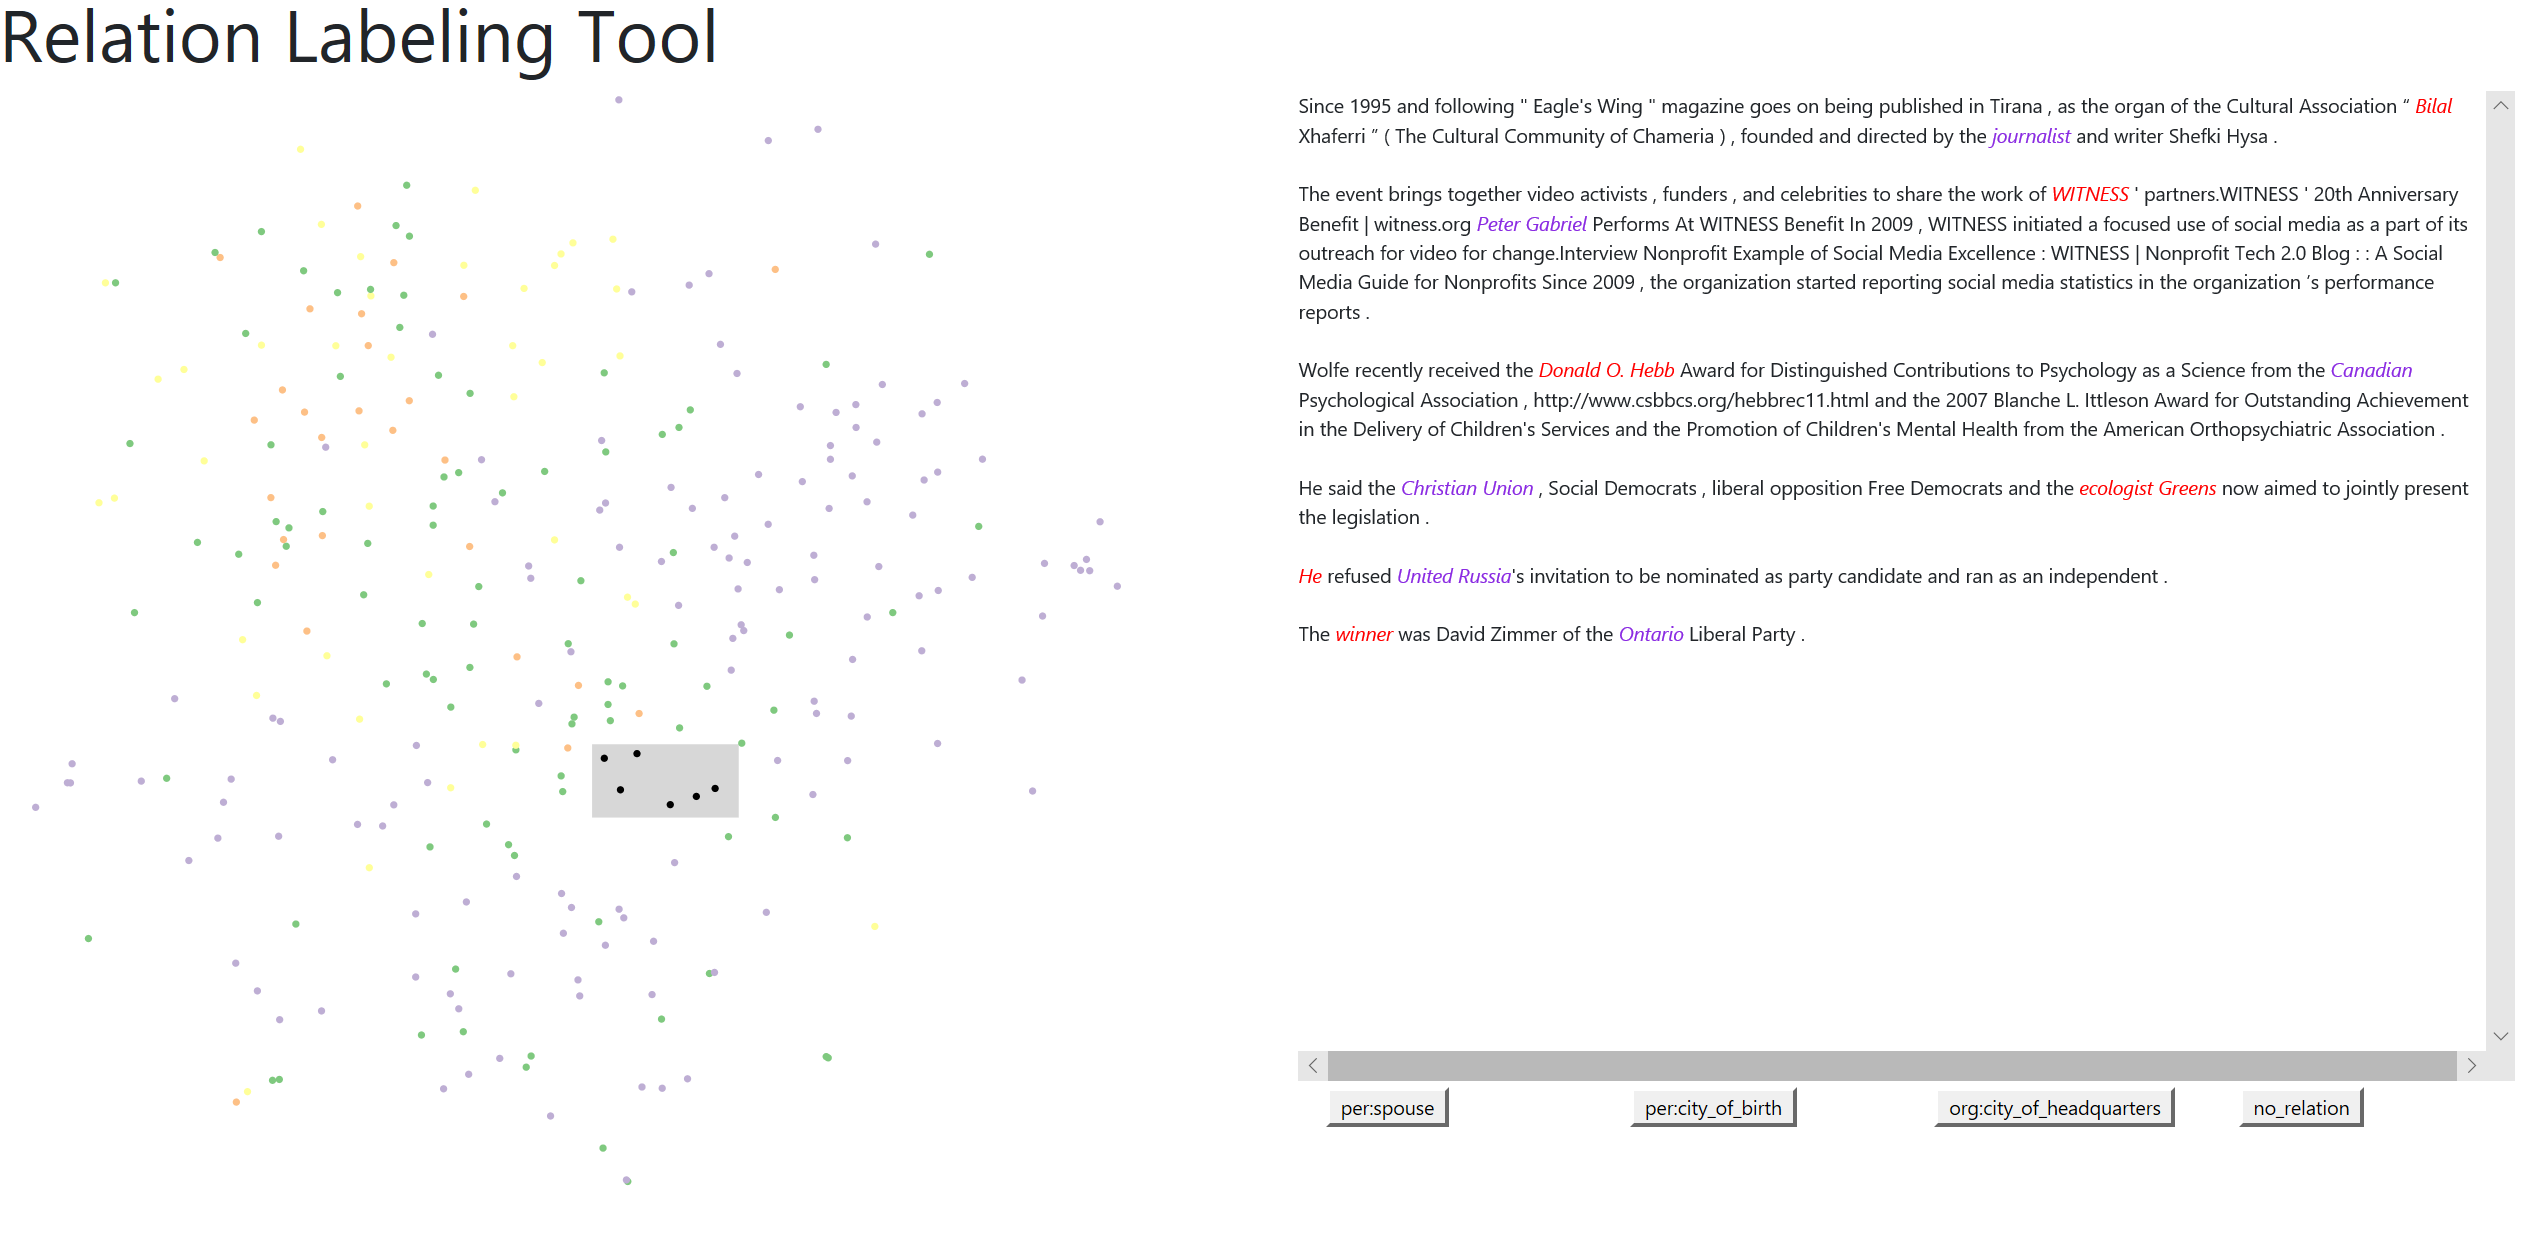
\includegraphics[width=\linewidth]{1.PNG}
  \caption{Overview of the Relation Labeling Tool. The left view shows the 2D projection of the sentences. The right view lists the sentences selected and allows the user to label them.}
  \label{fig:1}
\end{figure}
	
	The Relation Labeling Tool and human labeling are incorporated into the MIML\_RE relation extraction model in the following steps:
	
	\begin{itemize}
		\item For each EM iteration, after the E-step the model will select certain number of candidates for user to label based on some active learning criterion.
		\item The Relation Labeling Tool will then process the candidates and project them into 2D. The candidates will be plotted onto the interface using a pre-defined color map that will help the user to select instances. i.e The 2D projection and the color map will ideally help the user identify classes and patterns.
		\item The user can click on data points to select a single instance or use a selection tool (rectangle or lasso) to select multiple instances. The original sentences of selected instances will be shown in the right view, with the underlying entity pair highlighted, and the user can select a proper relation label or ``no relation'' for the instances.
		\item The results of user selection will be sent back to the model and be viewed as hard labeled data that cannot be changed by later E-steps.
		\item The process repeats for a few times until the model is trained.
	\end{itemize}
	
	Several active learning strategies for relation extraction are considered in ~\citet{angeli2014combining}. However, the results of their experiment may not hold in our case because the number of candidates are reduced and the candidates may not have a good 2D projection, i.e. the classes might not be sufficiently distinguishable in 2D projections. In their experiments their active learning models selected over 30,000 instances for crowdsourced annotation, while in our study the number of instances that the user can annotate is limited due to time and resources available.
	
	A key component of the Relation Labeling Tool is projecting the data instances to 2D. This consists of two steps. The first is to construct a vector representation for each sentence i.e. sentence embedding. Then we can apply a dimensionality reduction method such as PCA, MDS, or T-SNE to project the instances. Selecting the right dimensionality reduction method is crucial to our tool because class separability of the plot greatly affects the users' selection ~\cite{bernard2018comparing}.
	
	Unlike the MNIST dataset tested in ~\cite{bernard2018comparing}, our data is textual and much more complicated. It will take longer for the user to label data and the accuracy of the annotations will be lower. 
	
	\section{Implementation Details and Experimental Results}
	
	Due to time limitations, only a primitive prototype of the Relation Labeling Tool is implemented. The tool is not yet connected and tested with the MIML\_RE model. Further experiments and user studies need to be done and improvements of the sentence embedding and data projection algorithms can be applied.
	
	\subsection{Development Data}
	Ideally the input data for Relation Labeling Tool should be the output of the active learning strategy applied to the E-step of the training model. However, the MIMR\_RE model in ~\citet{surdeanu2012multi} used sophisticated features extracted from a custom corpora, and the original sentences are not provided with their training data. Therefore, for development purpose, we used labeled sentences from ~\citet{angeli2014combining}. There are in total 33,814 labeled sentences and 42 relation categories including ``no relation''. To simplify the problem, we manually select 3 categories ``per:spouse'', "per:city\_of\_birth", ``org:city\_of\_headquarters'' plus ``no relation'' and randomly sample 300 instances from the labeled sentences as candidate instances. The number of ``no relation'' instances sampled is proportional to the ratio of negative samples in the whole data.
	
	We acknowledge that this development dataset could be problematic, in that the real candidates from the active learning strategy could be vastly different from our random samples. The ratio of negative samples could also be different. Moreover, We didn't consider all the categories due to complexity, but the usefulness of the Relation Labeling Tool designed for small number of categories could decrease dramatically when the data is more complicated.
	
	\subsection{Sentence Embedding and 2D Projection}
	To present the candidate instances as 2D plots we need to encode them into vectors in order to apply a dimensionality reduction algorithm. As discussed in the previous section, this is the key part of Relation Labeling Tool. 
	
	There are multiple ways to construct sentence embedding. A good starting point is the weighted average bag-of-words algorithm from ~\citet{arora2016simple}, although a supervised method might have better results. It is also possible to construct sentence embedding using the features used by ~\citet{surdeanu2012multi} which has rich information on the syntactic structures of the sentences. In our experiments, we implemented the bag-of-words algorithm from ~\citet{arora2016simple}, and we estimated word frequencies using the development data.
	
	For dimentionality reduction, T-SNE generally yields better results in terms of class separability. It's the default method implemented in our tool.
	
	Figure ~\ref{fig:2} shows the results of the 2D projection for 4 different samples. The data points are colored by their true labels. From the plots we can see that although data instances from the same categories tend to be grouped together, the classes are hardly separated, and instances with ``no relation'' tend to scatter all over the space. In reality, we can only color the data points by their projected label from the model, and it could make the colormap even worse.
	
\begin{figure}[!htbp]
  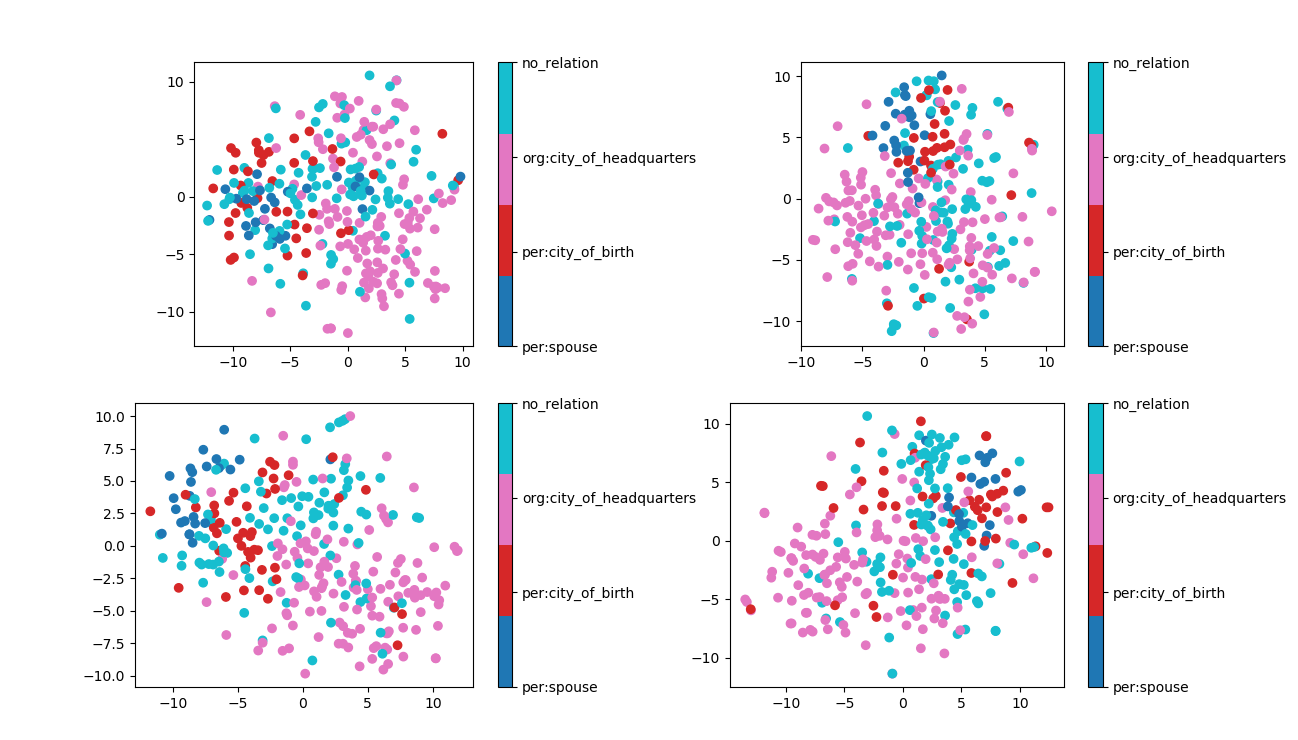
\includegraphics[width=\linewidth]{2.PNG}
  \caption{Results of 2D projection for 4 different samples, colormapped by the true label of the instances.}
  \label{fig:2}
\end{figure}

\subsection{Visual Labeling Interface}

Finally the projected candidate instances can be viewed in the Relation Labeling Tool interface showed in Figure ~\ref{fig:1} and the user can select single or multiple instances using a rectangle tool. The original sentence of the selected instances are shown with the entity pair highlighted. 

The Relation Labeling Tool is a web-based interface developed using \texttt{D3.js}. Due to the complexity of the textual data, the interface combines the scatter-plot view and the list view for easier annotation. The list view from ~\citet{angeli2014combining} has the most probable relation labels predicted by the model as choices for the user, which is not implemented in our tool. This can be implemented as future work. However, for multi-instance labeling, this could cause the interface to be crowded.

In our experiment, the data instances are colored by their true label, which is not possible in real training scenarios where the true labels are unknown. We could color the data points by the predicted label from the model, or we could use a 2D positional colormap independent of the model. User study is needed to verify which colormap scheme is the best for the task.

\section{Conclusion}

This project aims to design and implement a visual interactive labeling tool for relation extraction, hoping to improve the efficiency and accuracy of human annotation for relation extraction. As seen in the previous sections, many future work is needed for this purpose. However, a basic framework for Relation Labeling Tool is implemented and some clear improvement paths are discovered from the experiments.

Firstly, an active learning strategy can be combined with the visual labeling tool to better select candidate instances. Which active learning strategy is best suited with the tool remains a future study project. Secondly, vector representation of the sentences needs to be carefully constructed so that the 2D projection can be more distinctive. More sophisticated features and sentence embedding models could be used instead of simple weighted bag-of-words. Different dimensionality reduction methods may also have an impact on the quality of 2D projection. Moreover, improvements can be done to the labeling interface regarding the colormap and sentence list view. Lastly, the experiments are only done on a small sub-sample of the dataset, with only 3 categories. The interface may need some major over-haul when more categories are considered.



  \bibliography{jiang_kairong_hw4}
  \bibliographystyle{acl_natbib_nourl}
  
  \end{document}
  